Ниже продемонстрированы результаты работы программного кода написанного на Python.


Потенциал из постановки задачи представлен на Рис.~\ref{fig:u0_x}.

\graphicspath{{../python_results}}

\begin{figure}[h]
\centering
    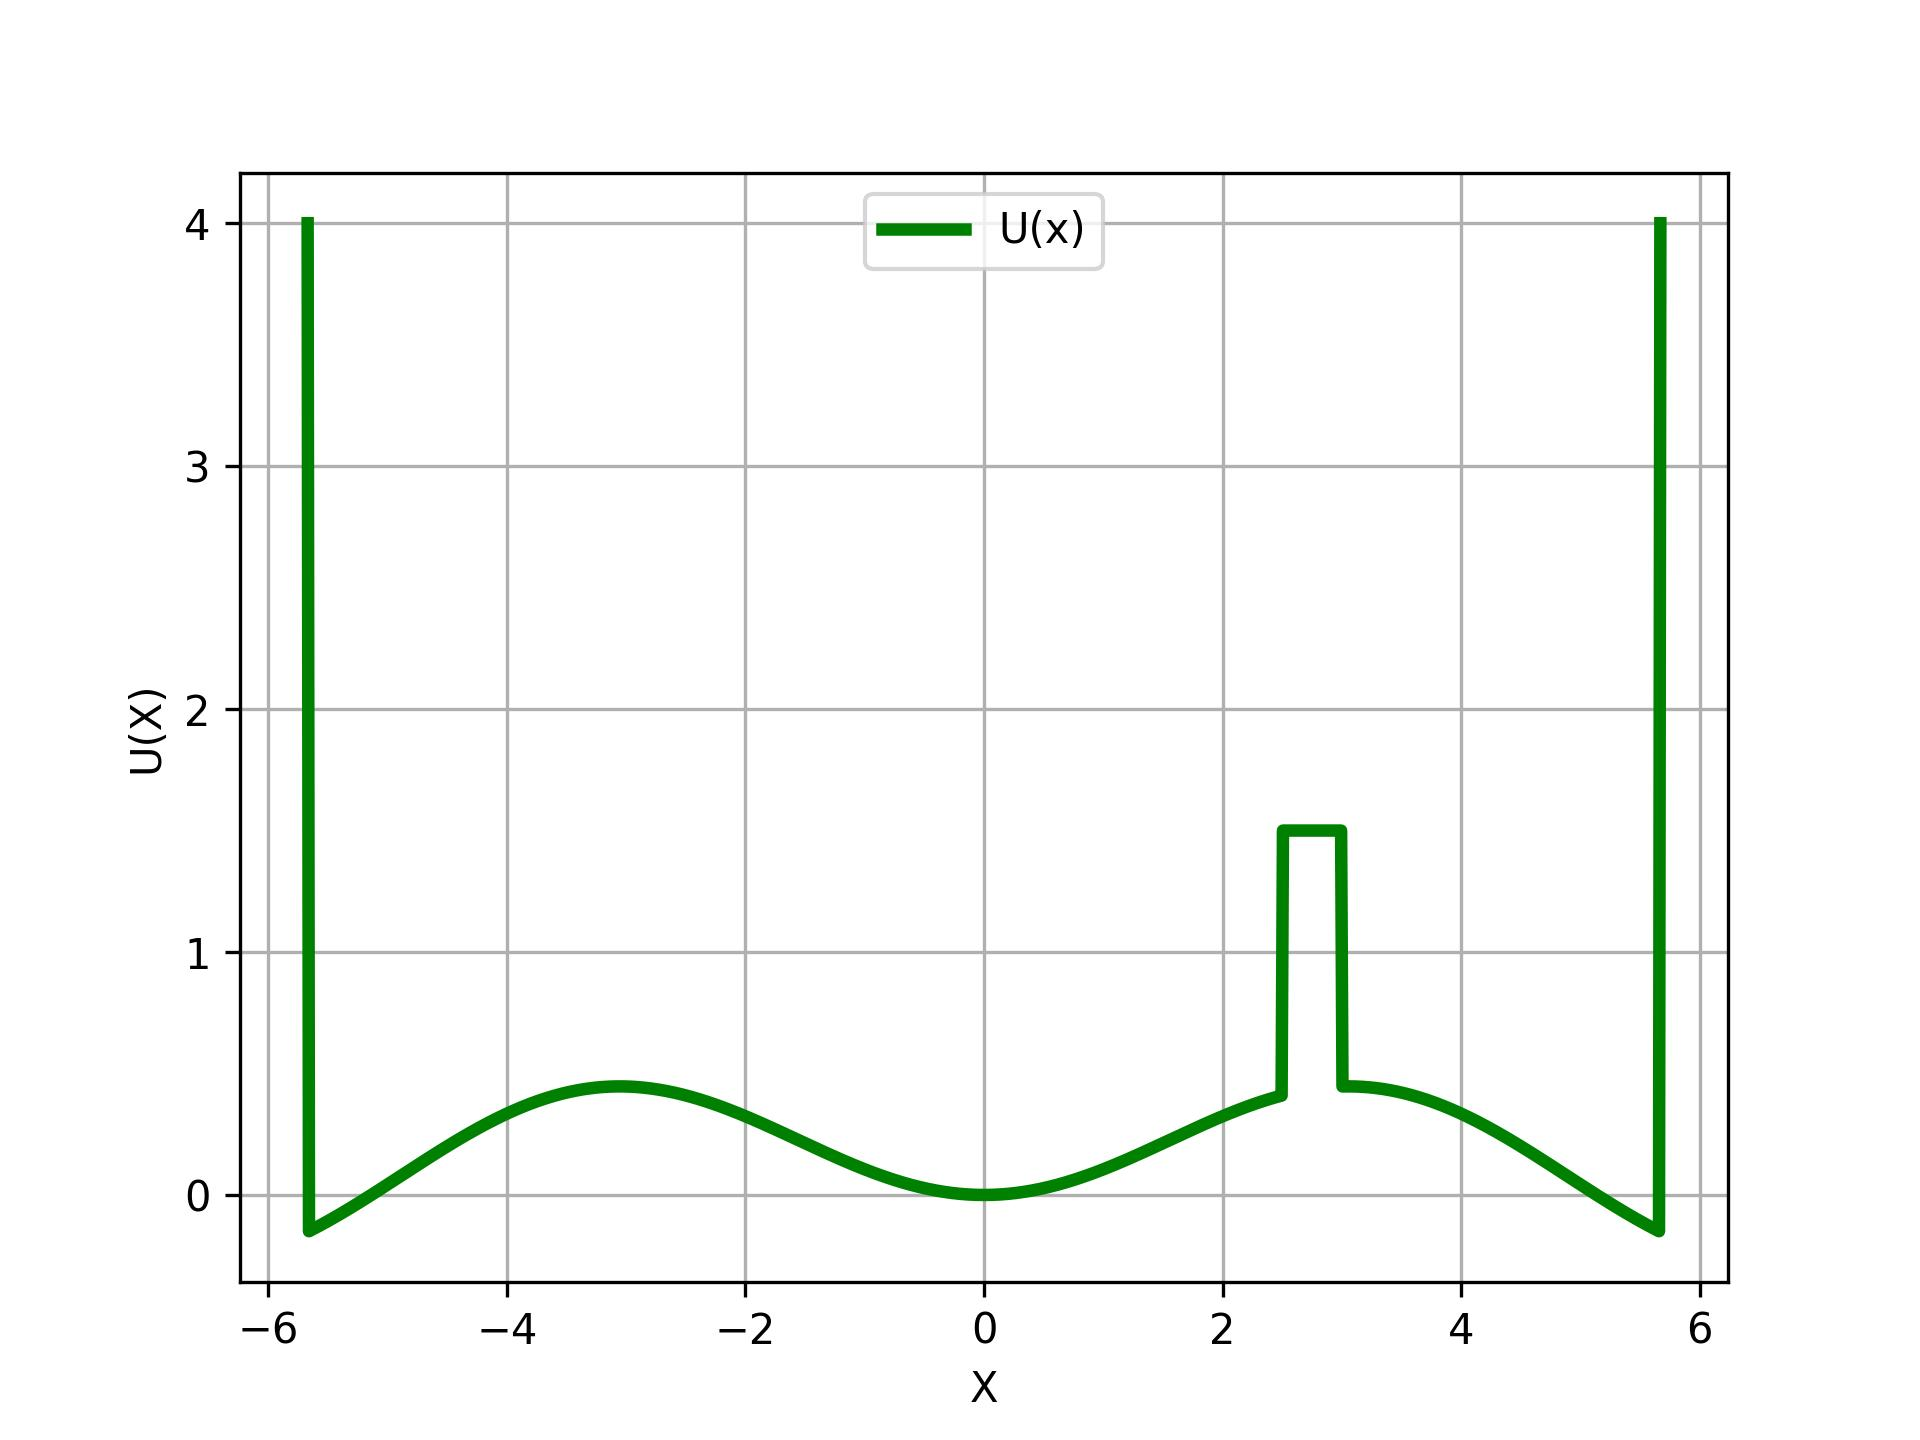
\includegraphics[width=0.8\linewidth]{U(X)}
    \caption{Невозмущенная система}\label{fig:u0_x}
\end{figure}

Возмущенная система представлена на Рис.~\ref{fig:u_x}.

\begin{figure}[h]
\centering
    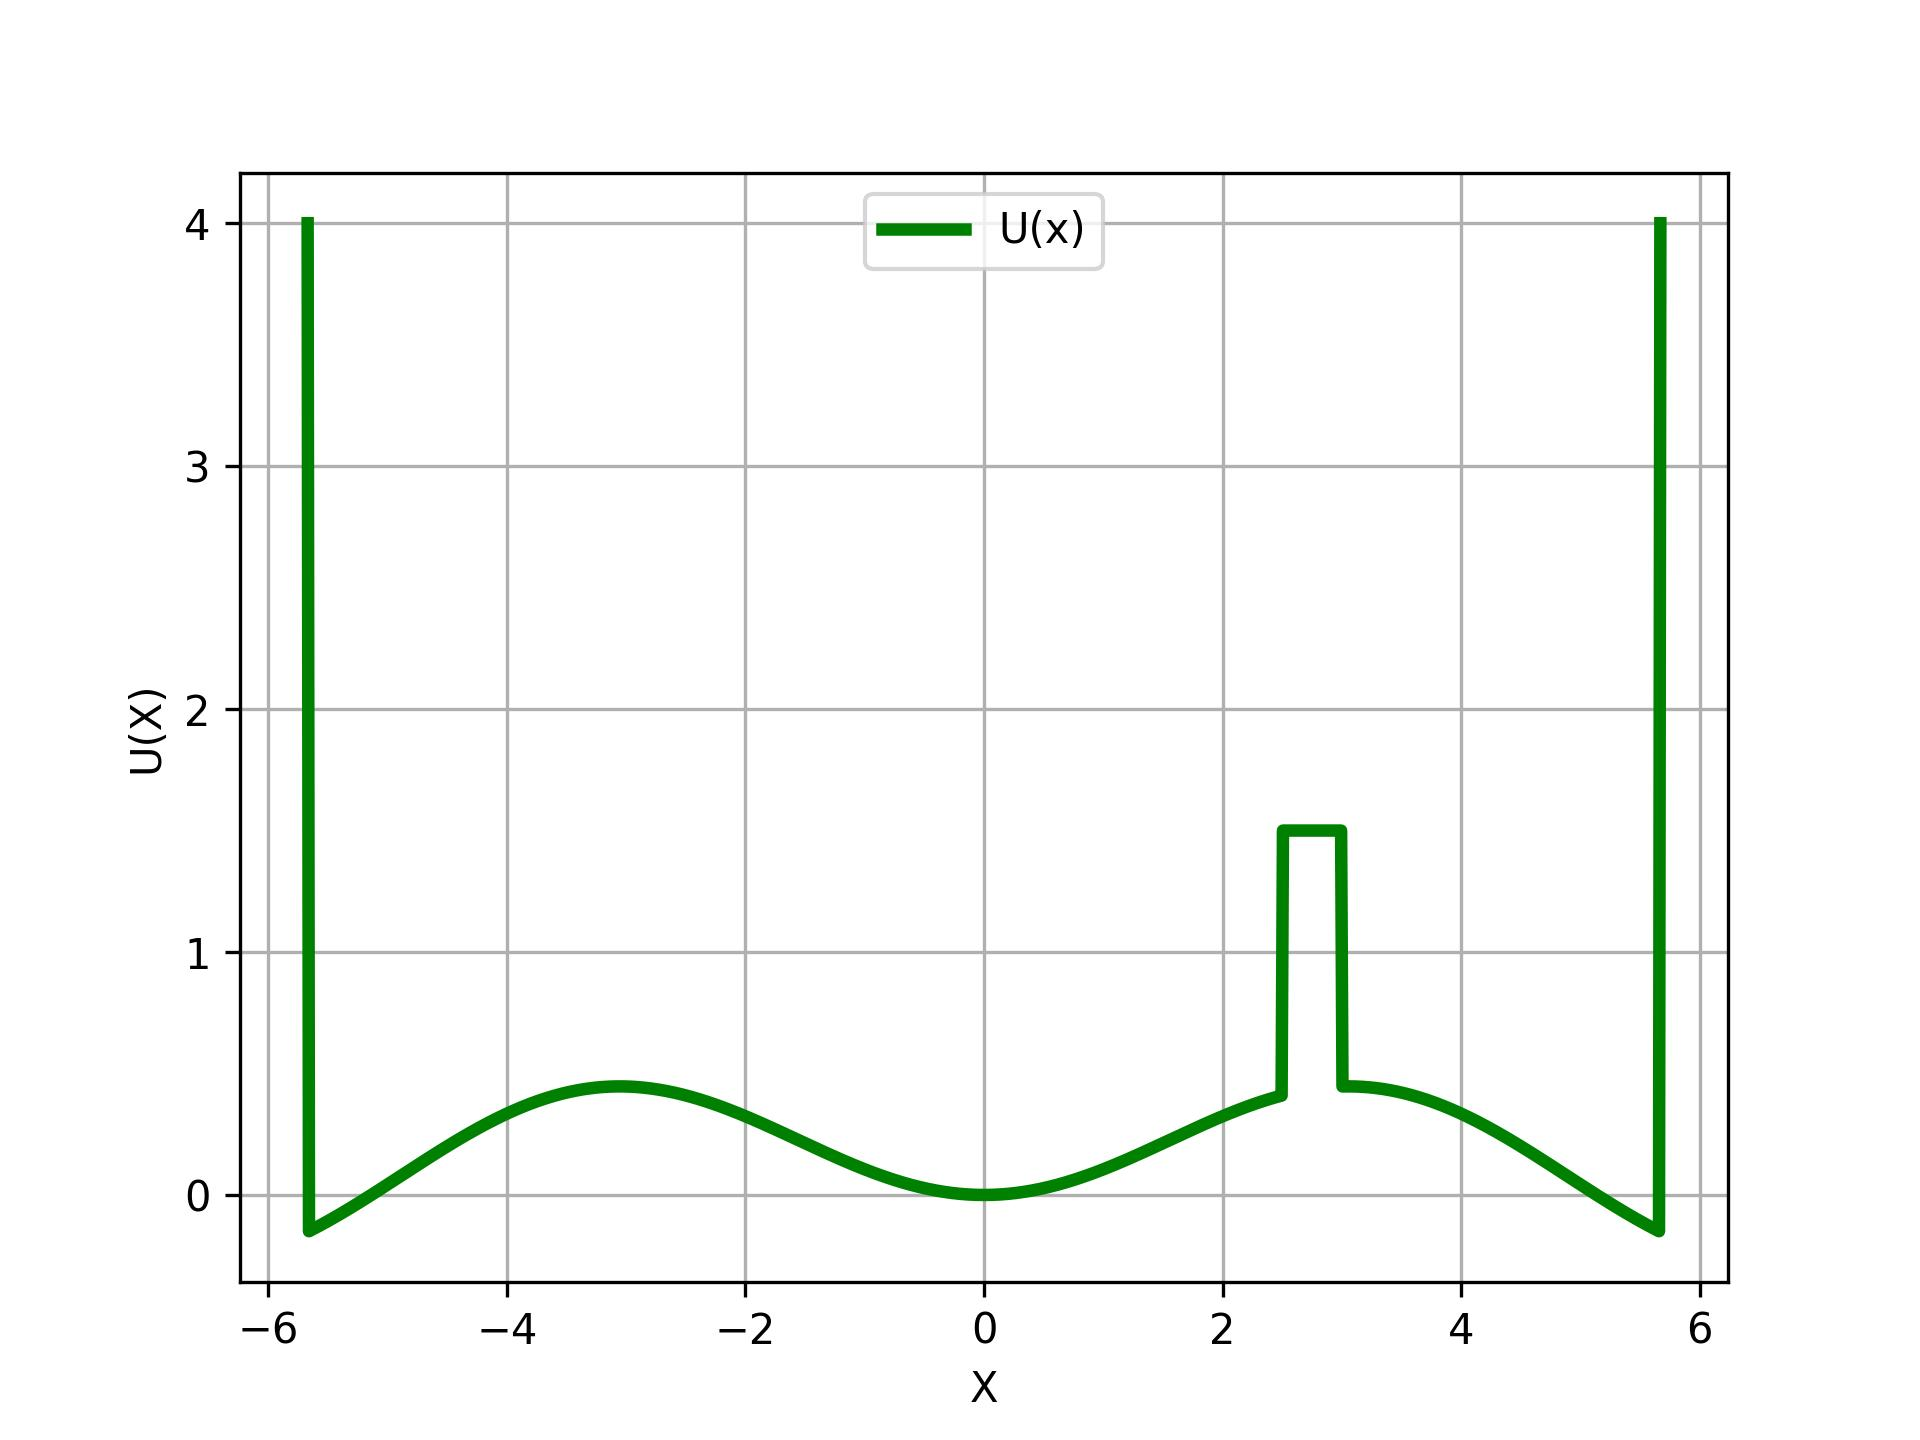
\includegraphics[width=0.8\linewidth]{U(X)}
    \caption{Возмущенная система}\label{fig:u_x}
\end{figure}

При вычислении энергии с учетом поправок для основного состояния возмущенной системы были получены следующие значения.


Энергии, где $e_0$ -- энергия основного состояния невозмущенной системы, а $e$ -- энергия возмущенной системы вычисленная с учетом поправок:

\begin{table}[H]
    \centering
    \begin{tabularx}{0.6\linewidth}{|X|X|}
        \hline
        \textbf{Энергия}&\textbf{а.е.} \\
        \hline
        $e_0$ & $0.026451$ \\
        \hline
        $e$ & $0.498856$ \\
        \hline
    \end{tabularx}
    \label{tab:sums0}
\end{table}

$s$ -- суммы из формулы второй поправки~\eqref{eq:EPsi_nk_first}, которая поочередно вычислялась с каждым состоянием невозмущенной системы:

\begin{table}[H]
    \centering
    \begin{tabularx}{0.8\linewidth}{|X|X|}
        \hline
        \textbf{Энергия невозмущенной системы}&\textbf{Энергия, а.е.} \\
        \hline
        1 & $-3.546785896711328e-14$ \\
        \hline
        2 & $-0.012860815109642064$ \\
        \hline
        3 & $-0.01286081510981086$ \\
        \hline
        4 & $-0.01286081510986983$ \\
        \hline
        5 & $-0.025191454299853946$ \\
        \hline
        6 & $-0.025191454299854834$ \\
        \hline
        7 & $-0.03018338913184664$ \\
        \hline
        8 & $-0.030183389131850178$ \\
        \hline
        9 & $-0.03177543923923762$ \\
        \hline
        10 & $-0.0317754392392409$ \\
        \hline
        11 & $-0.032087871459281776$ \\
        \hline
    \end{tabularx}
    \label{tab:energies_012}
\end{table}

На Рис.~\ref{fig:State0PB} представлена волновая функция и плотность вероятности возмущенной системы для основного состояния.

\begin{figure}[H]
\centering
    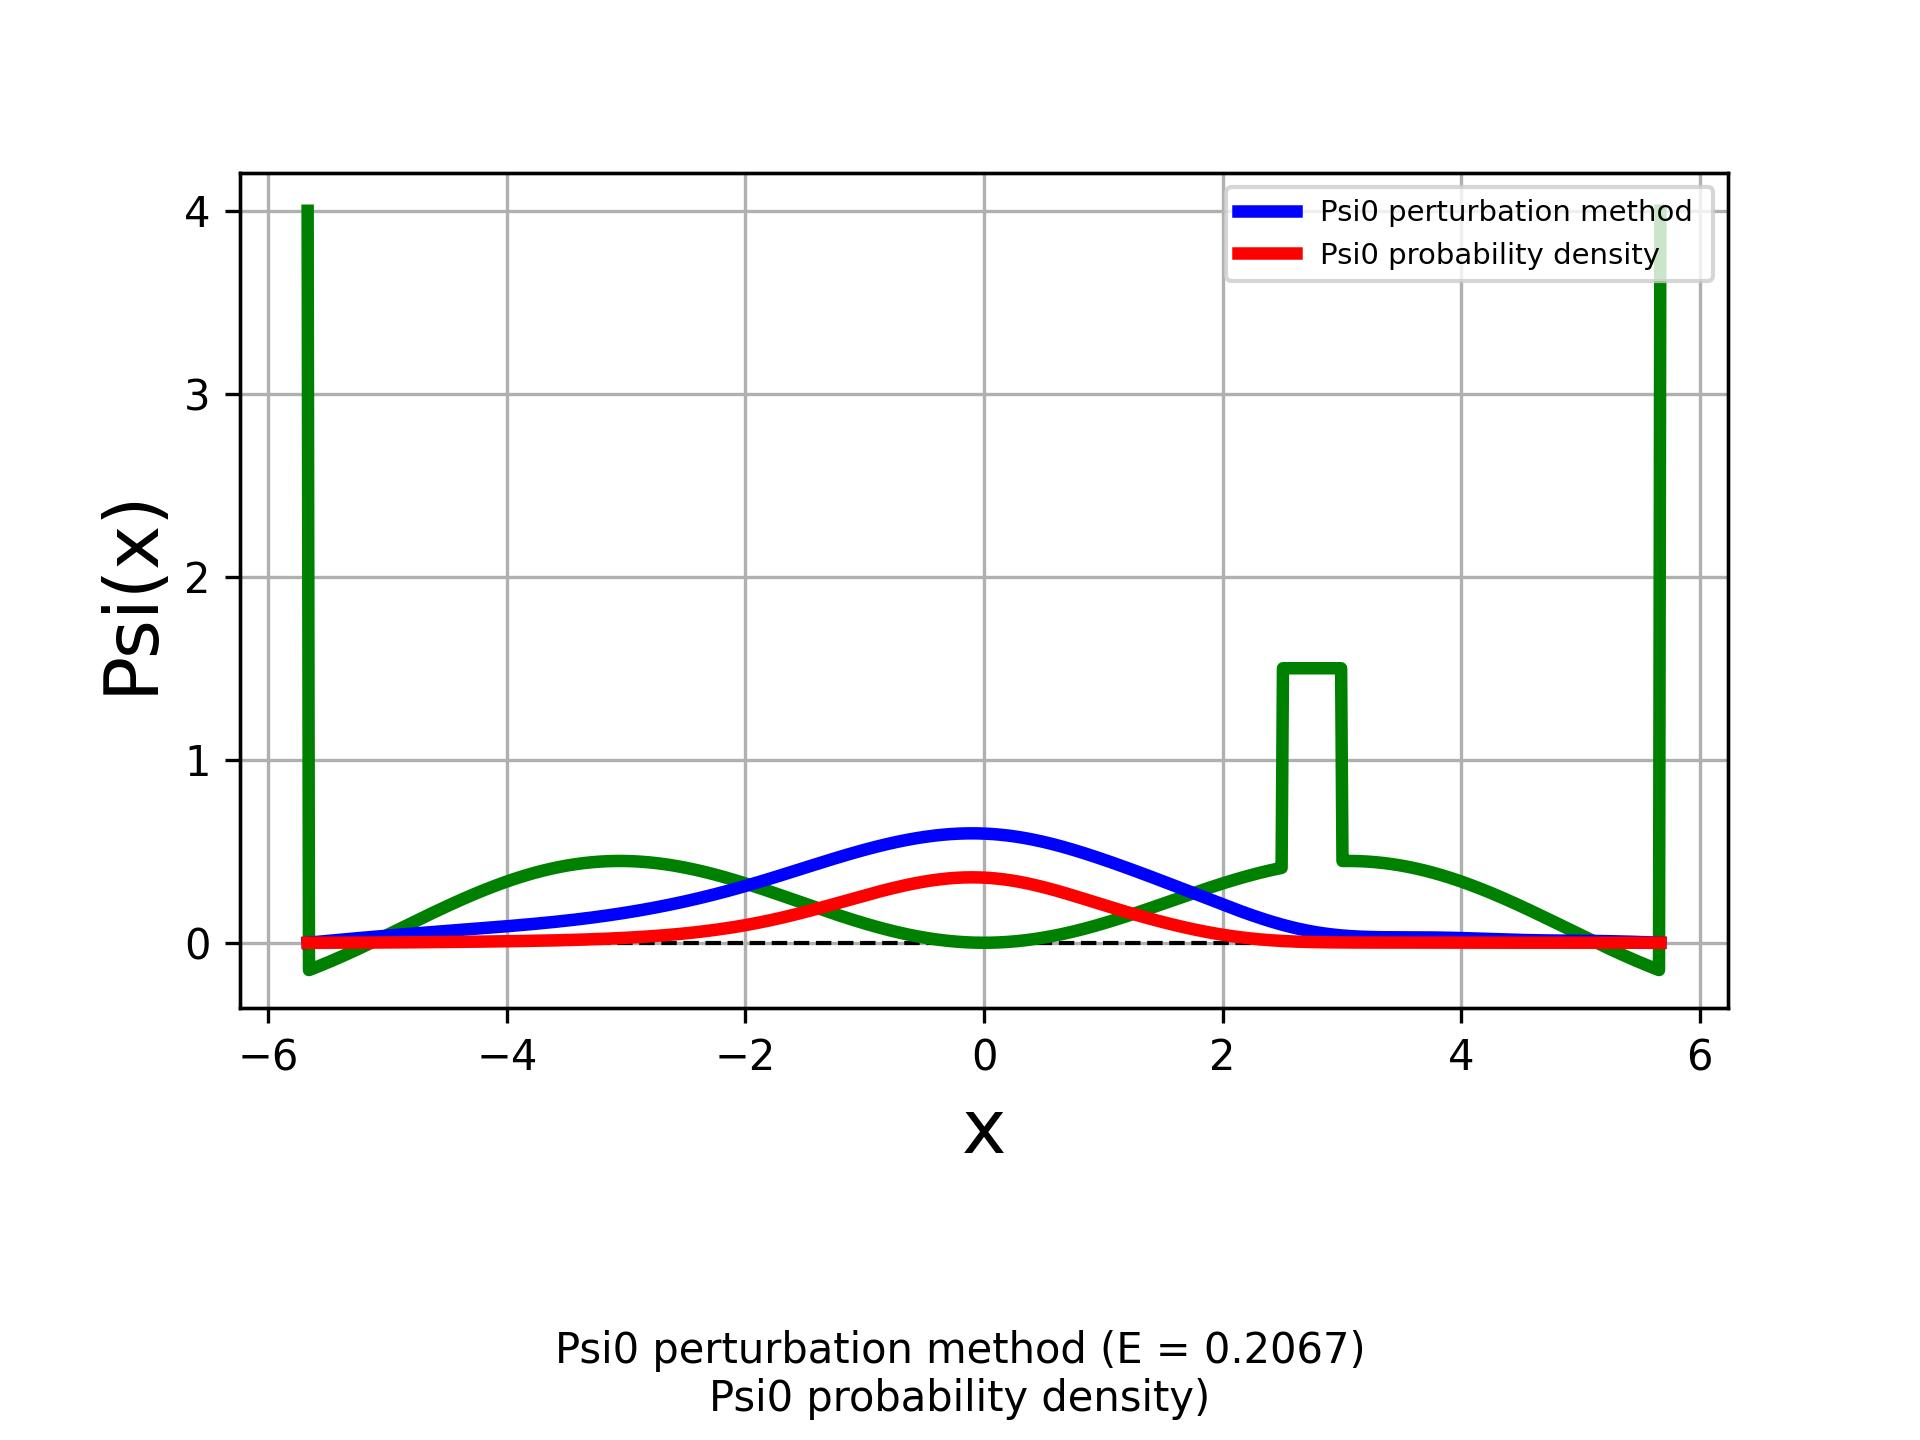
\includegraphics[width=0.75\linewidth]{State0 probability density}
    \caption{Волновая функция основного состояния возмущенной системы}\label{fig:State0PB}
\end{figure}

Данная функция соответствует основному состоянию осцилляционной теоремы.
Т.к, как уже было установленно в первой лабораторной работе,
основным состоянием в случае данной функции является состояние в котором волновая функция имеет два пересечения с осью абсцисс.


На Рис.~\eqref{fig:State0} представлено сравнение волновых функций основного состояния возмущенной системы вычисленных методом пристрелки и методом возмущений.


\begin{figure}[H]
\centering
    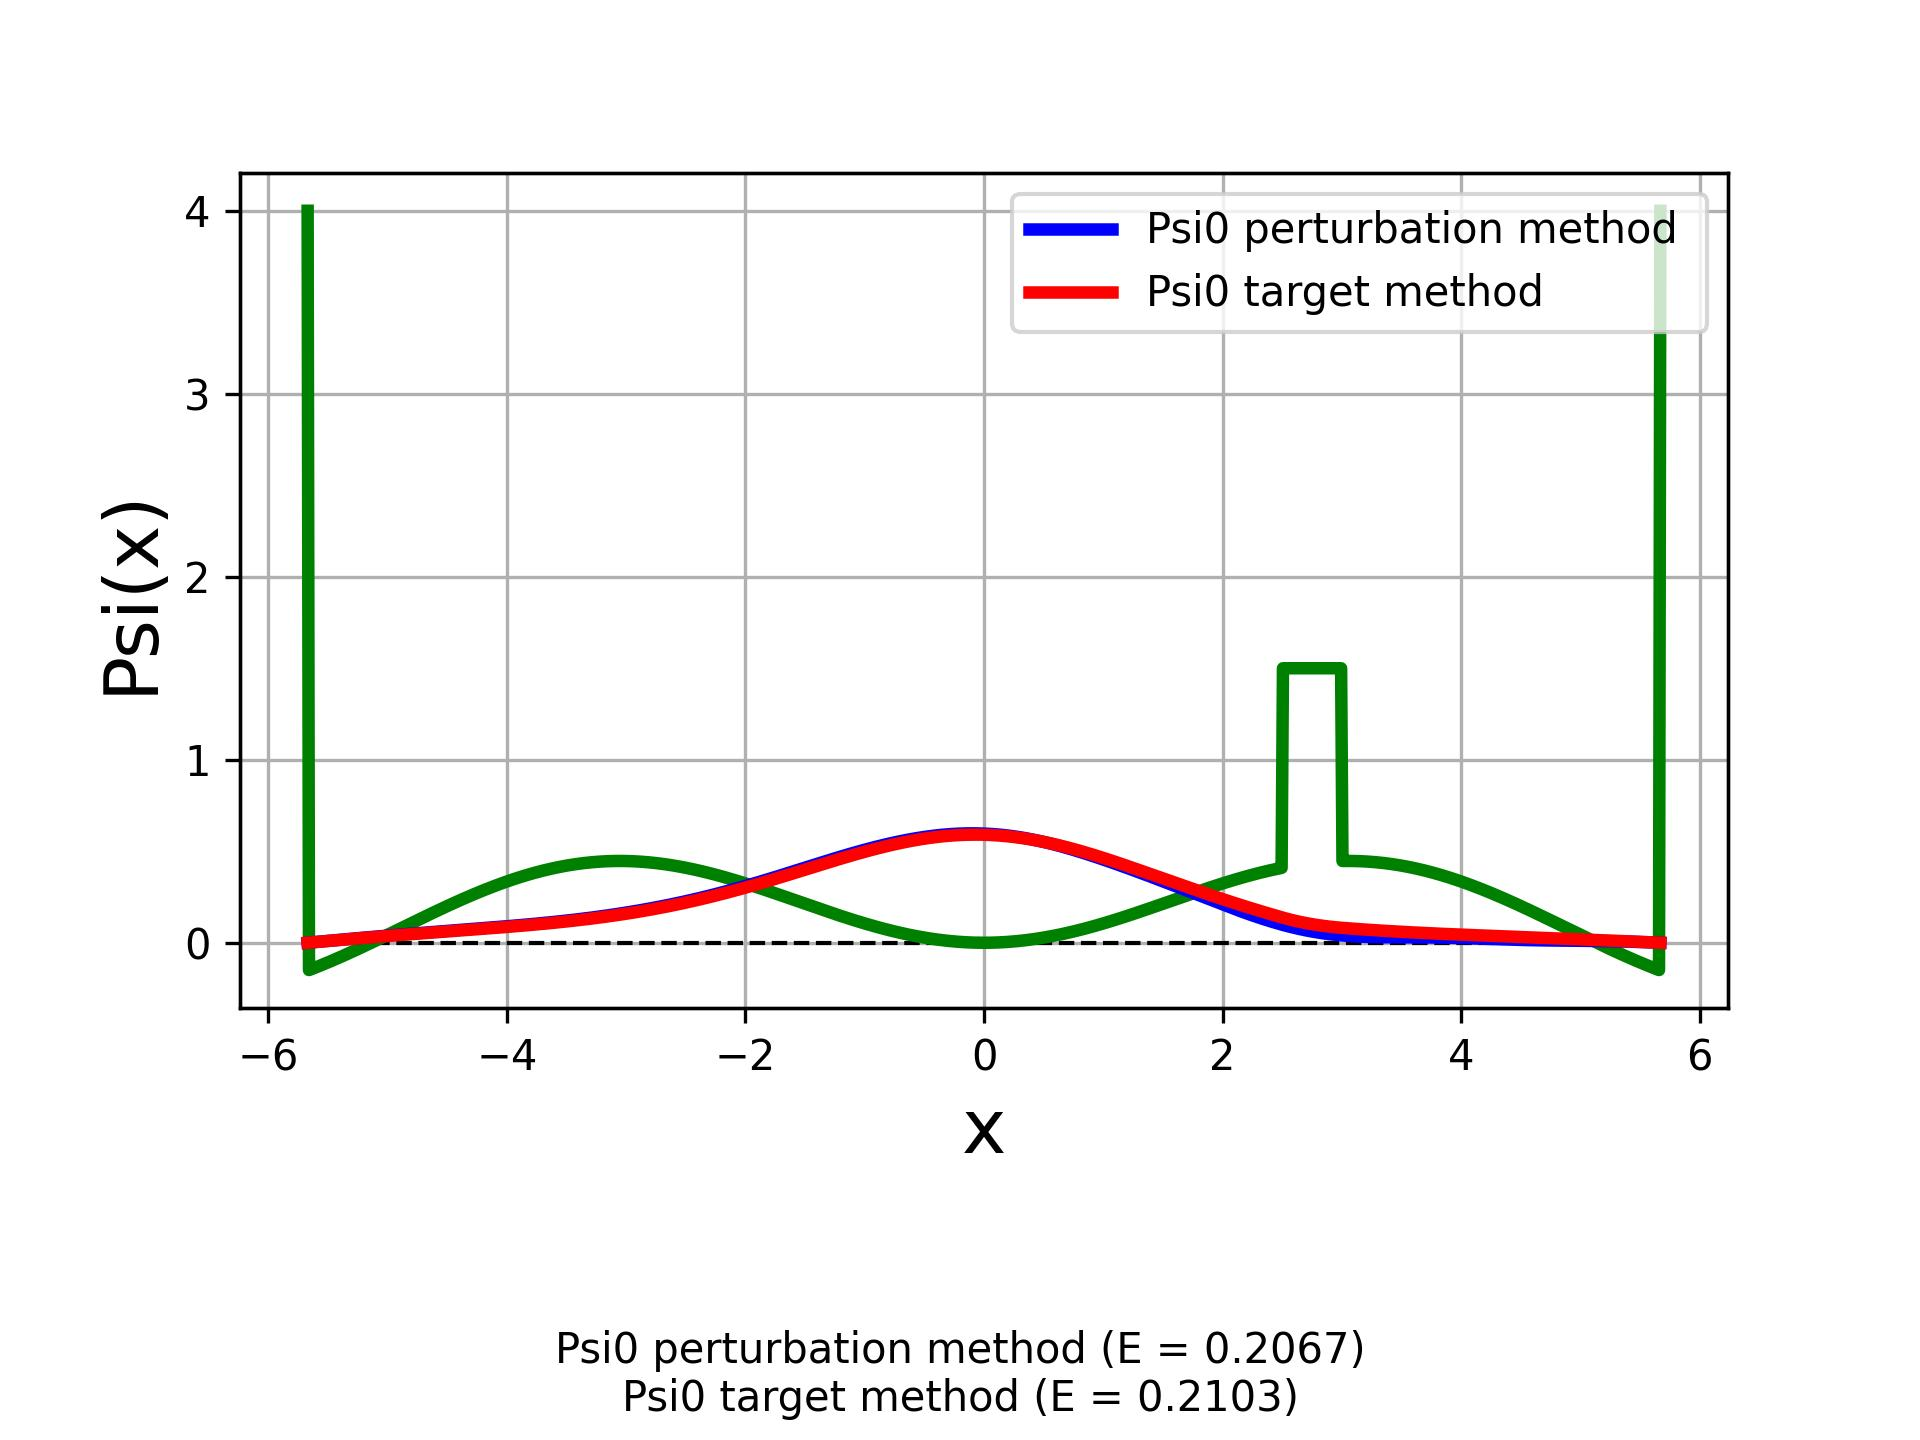
\includegraphics[width=0.75\linewidth]{State0}
    \caption{Сравнение волновых функций полученных разными методами}\label{fig:State0}
\end{figure}


Ниже представлены значения энергий основного состояния и квантовомеханических средних $\langle p(x) \rangle$ и $\langle p(x^2) \rangle$,
вычисленные методом пристрелки и методом возмущений:


\noindent
\begin{tabularx}{\linewidth}{|c|X|X|X|}
    \hline
    \textbf{Метод решения}&\textbf{Энергия, а.е.}&\textbf{$\langle p(x) \rangle$}&\textbf{$\langle p(x^2) \rangle$} \\
    \hline
    Метод возмущений & $0.339903$ & $0.000000e+00$ & $4.420559e-01$\\
    \hline
    Метод пристрелки & $0.302288$ & $0.000000e+00$ & $3.434077e-01$\\
    \hline
\end{tabularx}


При вычислении энергии с учетом поправок для второго возбужденного состояния возмущенной системы были получены следующие значения.


Энергии, где $e_0$ -- энергия второго возбужденного состояния невозмущенной системы, а $e$ -- энергия возмущенной системы вычисленная с учетом поправок:

\begin{table}[H]
    \centering
    \begin{tabularx}{0.6\linewidth}{|X|X|}
        \hline
        \textbf{Энергия}&\textbf{а.е.} \\
        \hline
        $e_0$ & $0.8155639648437506$ \\
        \hline
        $e$ & $0.8450739082702535$ \\
        \hline
    \end{tabularx}
    \label{tab:sums2}
\end{table}

$s$ -- суммы из формулы второй поправки~\eqref{eq:EPsi_nk_first}, которая поочередно вычислялась с каждым состоянием невозмущенной системы:

\begin{table}[H]
    \centering
    \begin{tabularx}{0.8\linewidth}{|X|X|}
        \hline
        \textbf{Энергия невозмущенной системы}&\textbf{Энергия, а.е.} \\
        \hline
        $0$& $0.012860815109606596$ \\
        \hline
        $1$& $0.012860815109628453$ \\
        \hline
        $3$& $0.012860815109407921$ \\
        \hline
        $4$& $0.012860815109389715$ \\
        \hline
        $5$& $0.011316012393792629$ \\
        \hline
        $6$& $0.011316012393790565$ \\
        \hline
        $7$& $0.01075306784158517$ \\
        \hline
        $8$& $0.010753067841582727$ \\
        \hline
        $9$& $0.010574304144826133$ \\
        \hline
        $10$ & $0.010574304144824201$ \\
        \hline
        $11$ & $0.010534361777482728$ \\
        \hline
    \end{tabularx}
    \label{tab:energies_212}
\end{table}


На Рис.~\ref{fig:State2PB} представлена волновая функция и плотность вероятности возмущенной системы для второго возбужденного состояния.


\begin{figure}[H]
\centering
    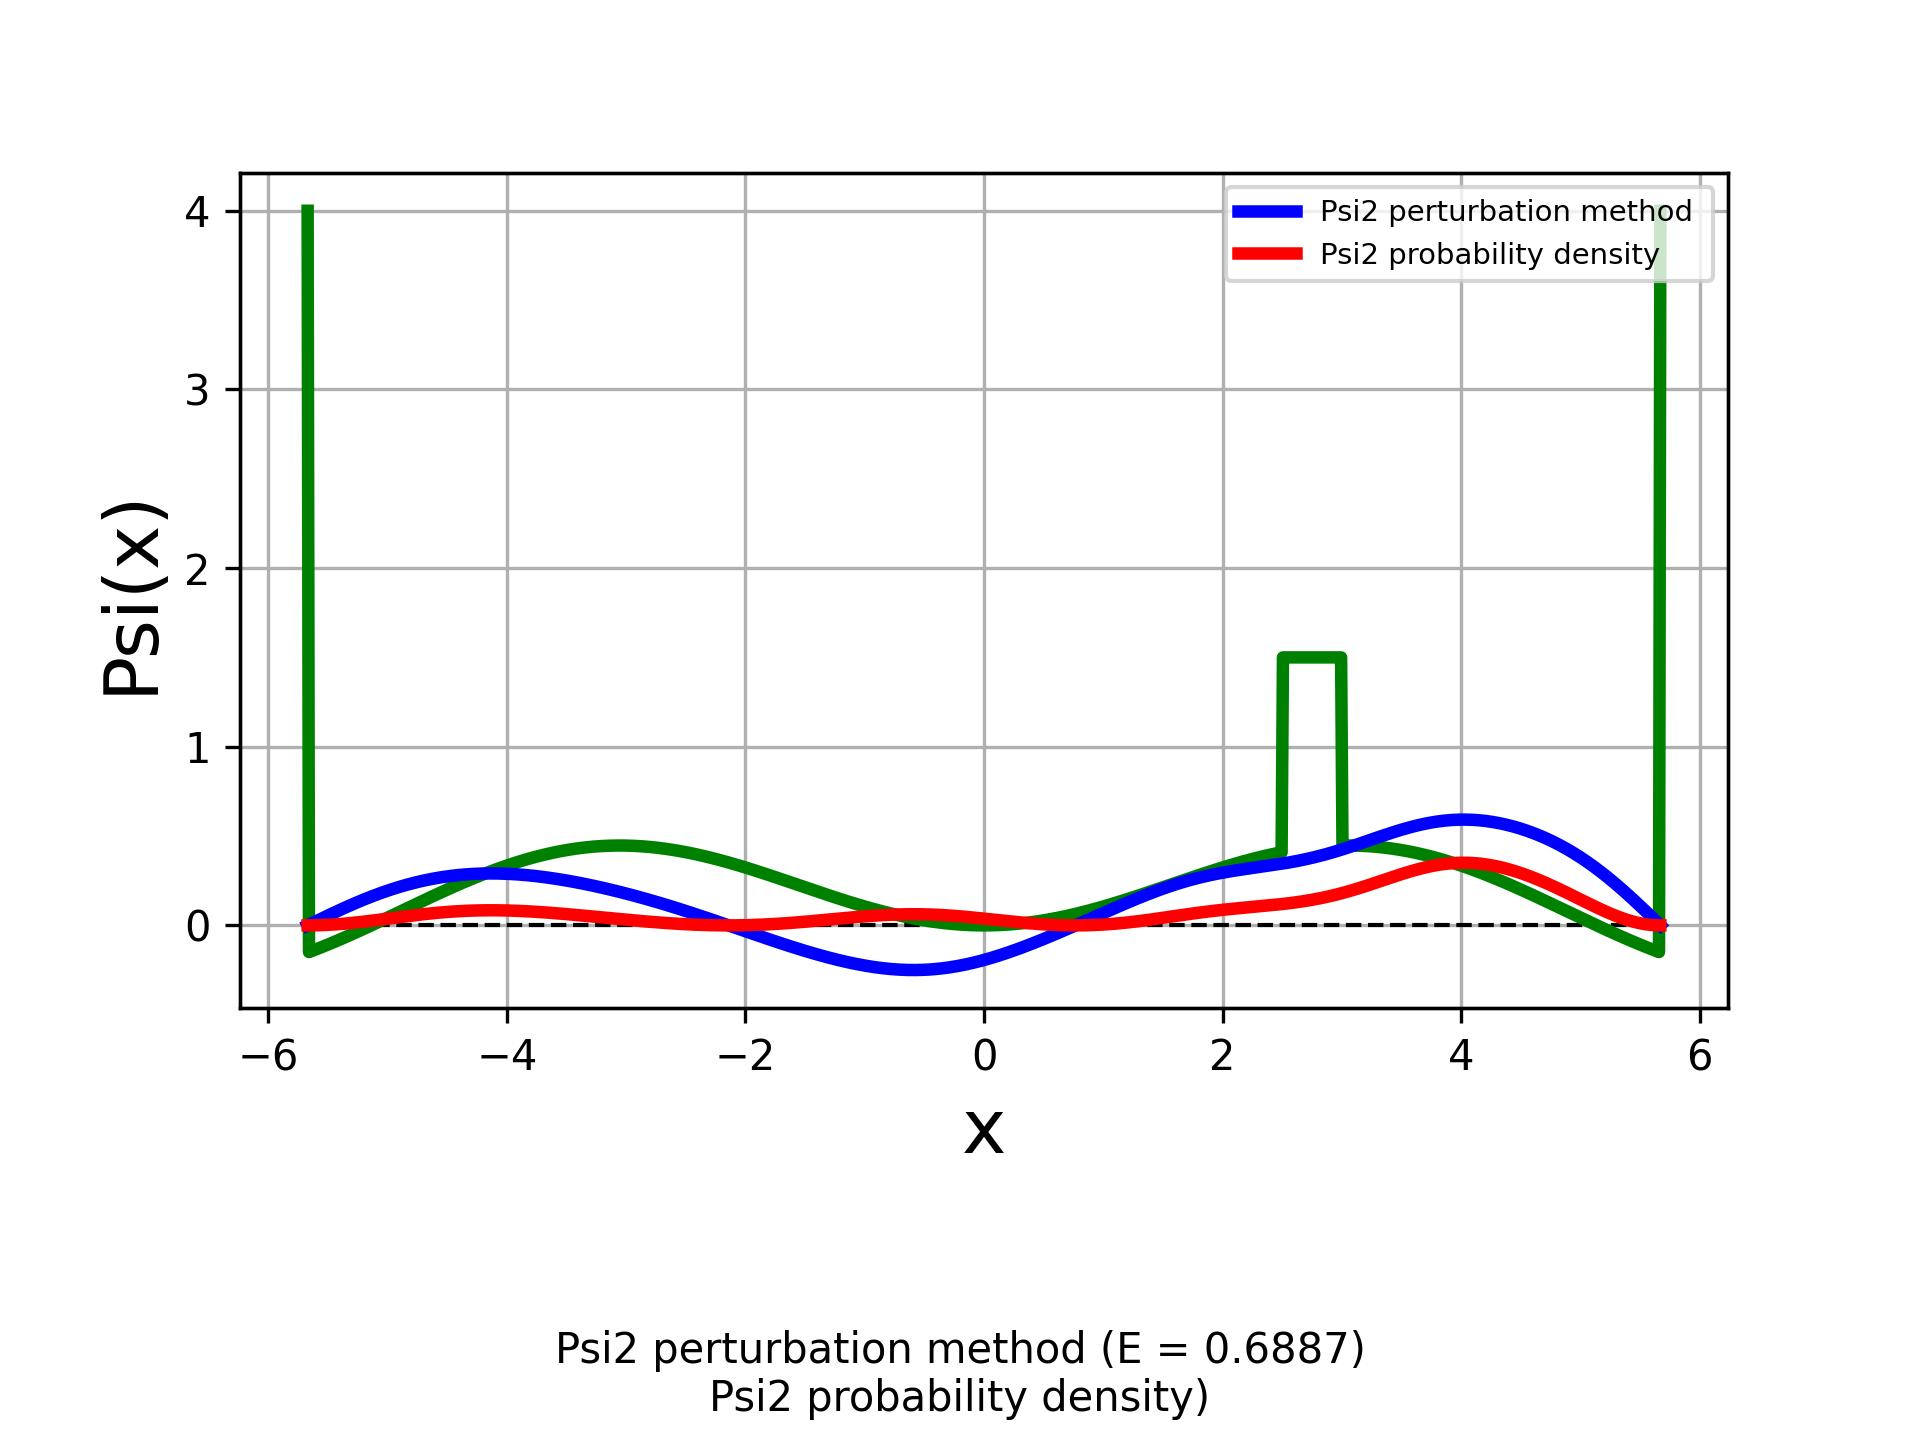
\includegraphics[width=0.75\linewidth]{State2 probability density}
    \caption{Волновая функция второго возбужденного состояния возмущенной системы}\label{fig:State2PB}
\end{figure}

Данная функция соответствует основному состоянию осцилляционной теоремы.
Т.к, как уже было установленно в первой лабораторной работе,
основным состоянием в случае функции основного состояния является состояние в котором волновая функция имеет два пересечения с осью абсцисс,
следовательно, для второго возбужденного имеется 4 пересечения с осью абсцисс.


На Рис.~\ref{fig:State2} представлено сравнение волновых функций второго возбужденного состояния возмущенной системы вычисленных методом пристрелки и методом возмущений.


\begin{figure}[H]
\centering
    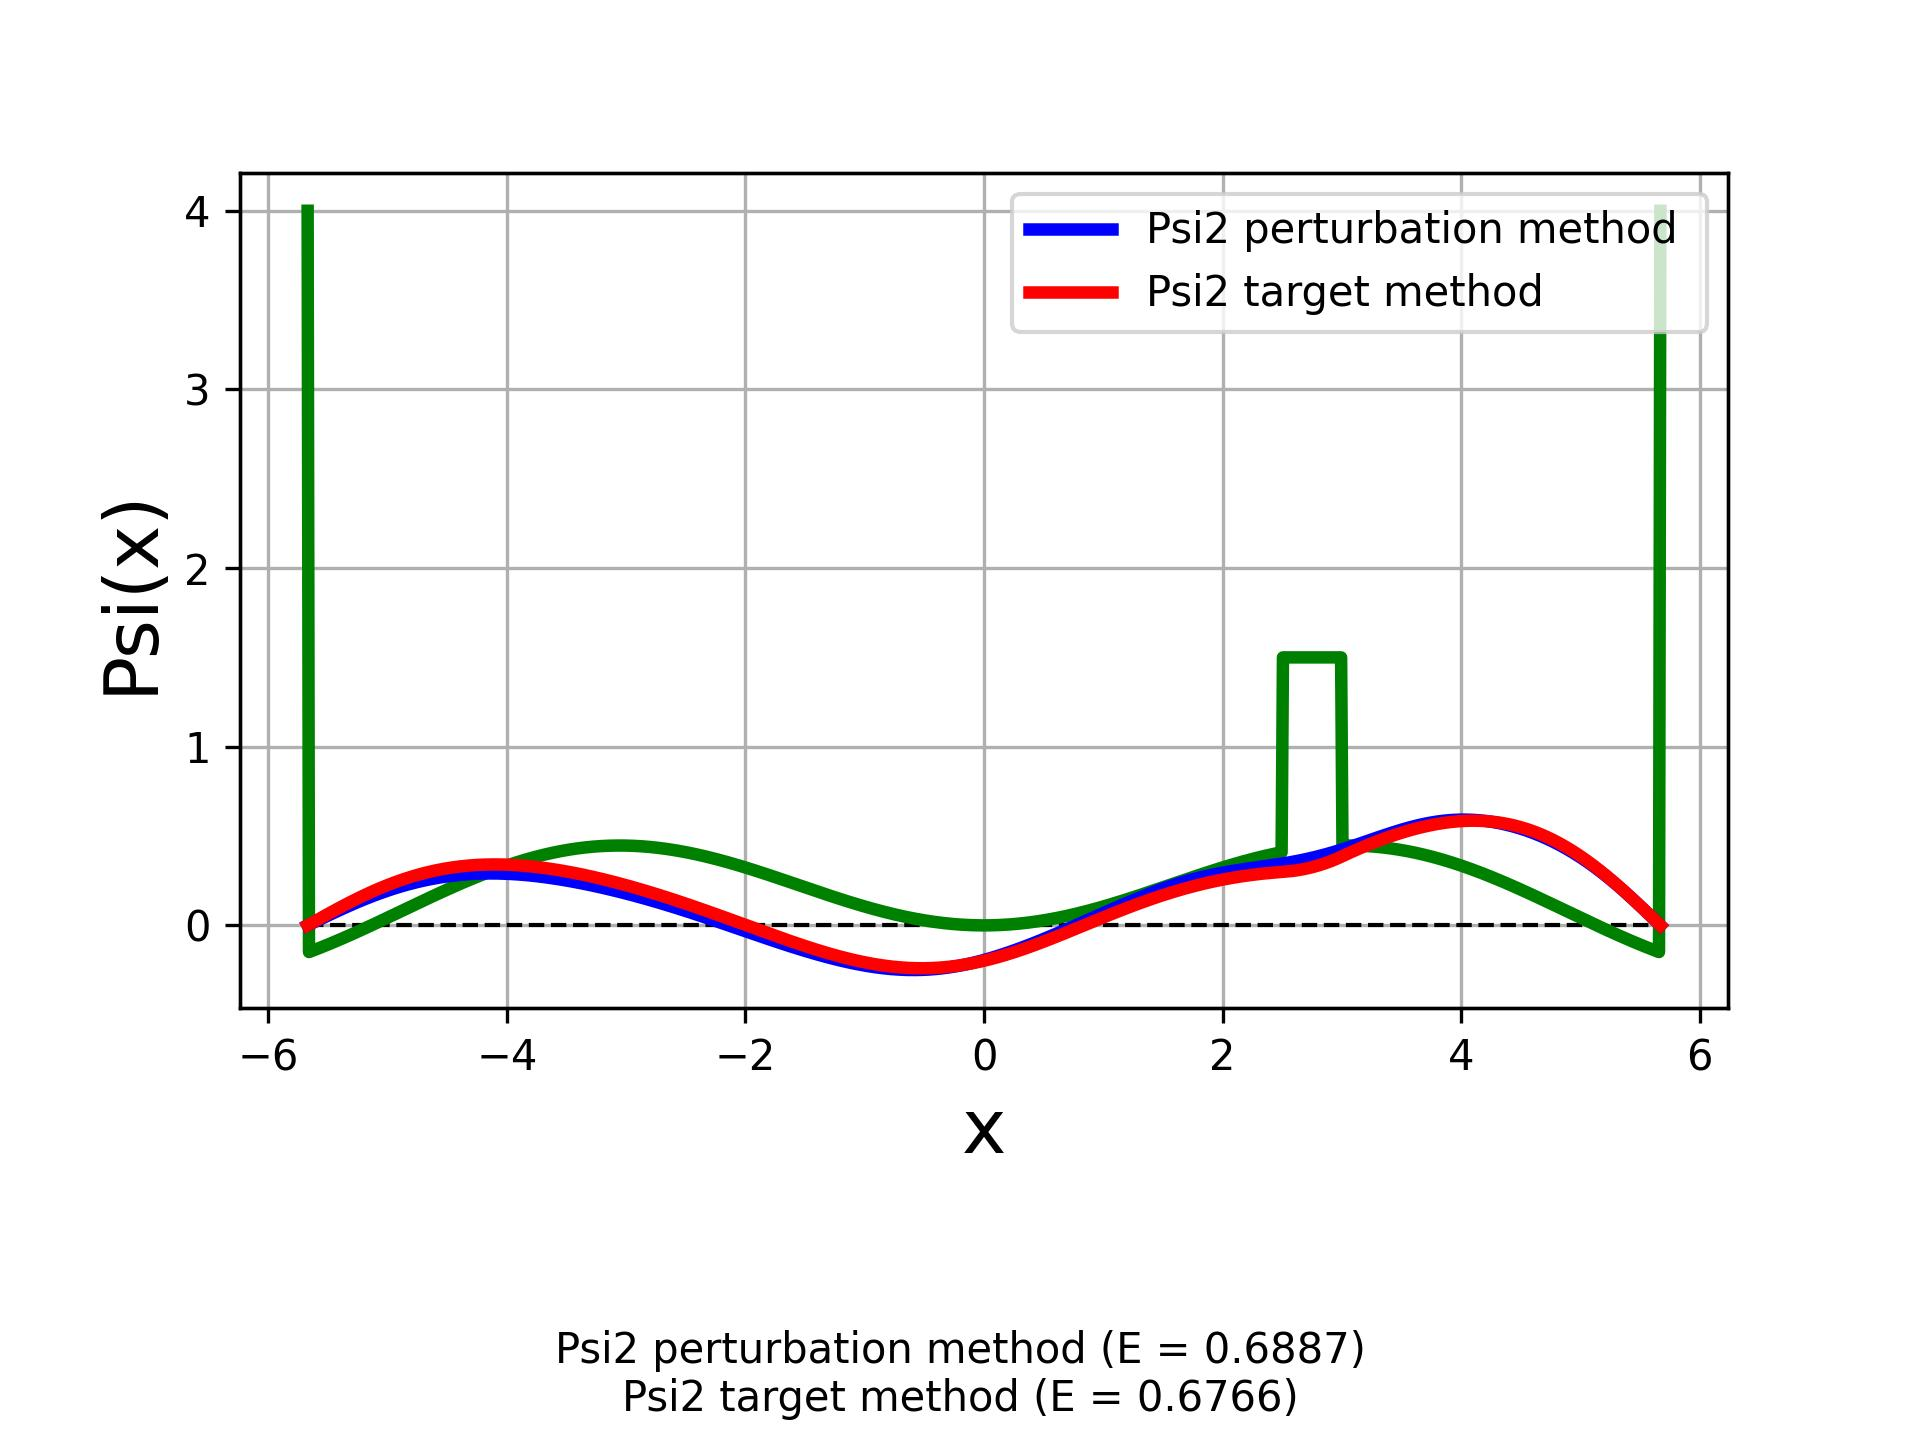
\includegraphics[width=0.75\linewidth]{State2}
    \caption{Сравнение волновых функций полученных разными методами}\label{fig:State2}
\end{figure}


Ниже представлены значения энергий второго возбужденного состояния и квантовомеханических средних $\langle p(x) \rangle$ и $\langle p(x^2) \rangle$,
вычисленные методом пристрелки и методом возмущений:


\noindent
\begin{tabularx}{\linewidth}{|c|X|X|X|}
    \hline
    \textbf{Метод решения}&\textbf{Энергия, а.е.}&\textbf{$\langle p(x) \rangle$}&\textbf{$\langle p(x^2) \rangle$} \\
    \hline
    Метод возмущений & $0.855608$ & $0.000000e+00$ & $2.374319e+00$\\
    \hline
    Метод пристрелки & $0.848595$ & $0.000000e+00$ & $2.649263e+00$\\
    \hline
\end{tabularx}
\newpage